\section{Installation and Architecture}
This project was developed using the React Javascript framework, with antlr4ts as an external parsing helper library. It is meant to run in the browser, and a public version can be accessed via this URL: \url{tinyurl.com/ocamltypechecker}. It accepts user input via a terminal-like interface where one line of input can be accepted at a time. When \verb|enter| is pressed, the input is put through our program and a valid type check output or an error output is presented in the subsequent line.

\subsection{Installation}
To test out our project locally, execute the following steps:
\begin{enumerate}
    \item Clone our repository \verb|ocaml-type-inference-in-ts| locally
    \item Run \verb|yarn install| in the root of the repository
    \item Run \verb|yarn start| in the root of the repository
    \item Open the local address address generated in your browser. You should see a frontend environment that looks like this: 
\end{enumerate}
\begin{figure}[H]
\centerline{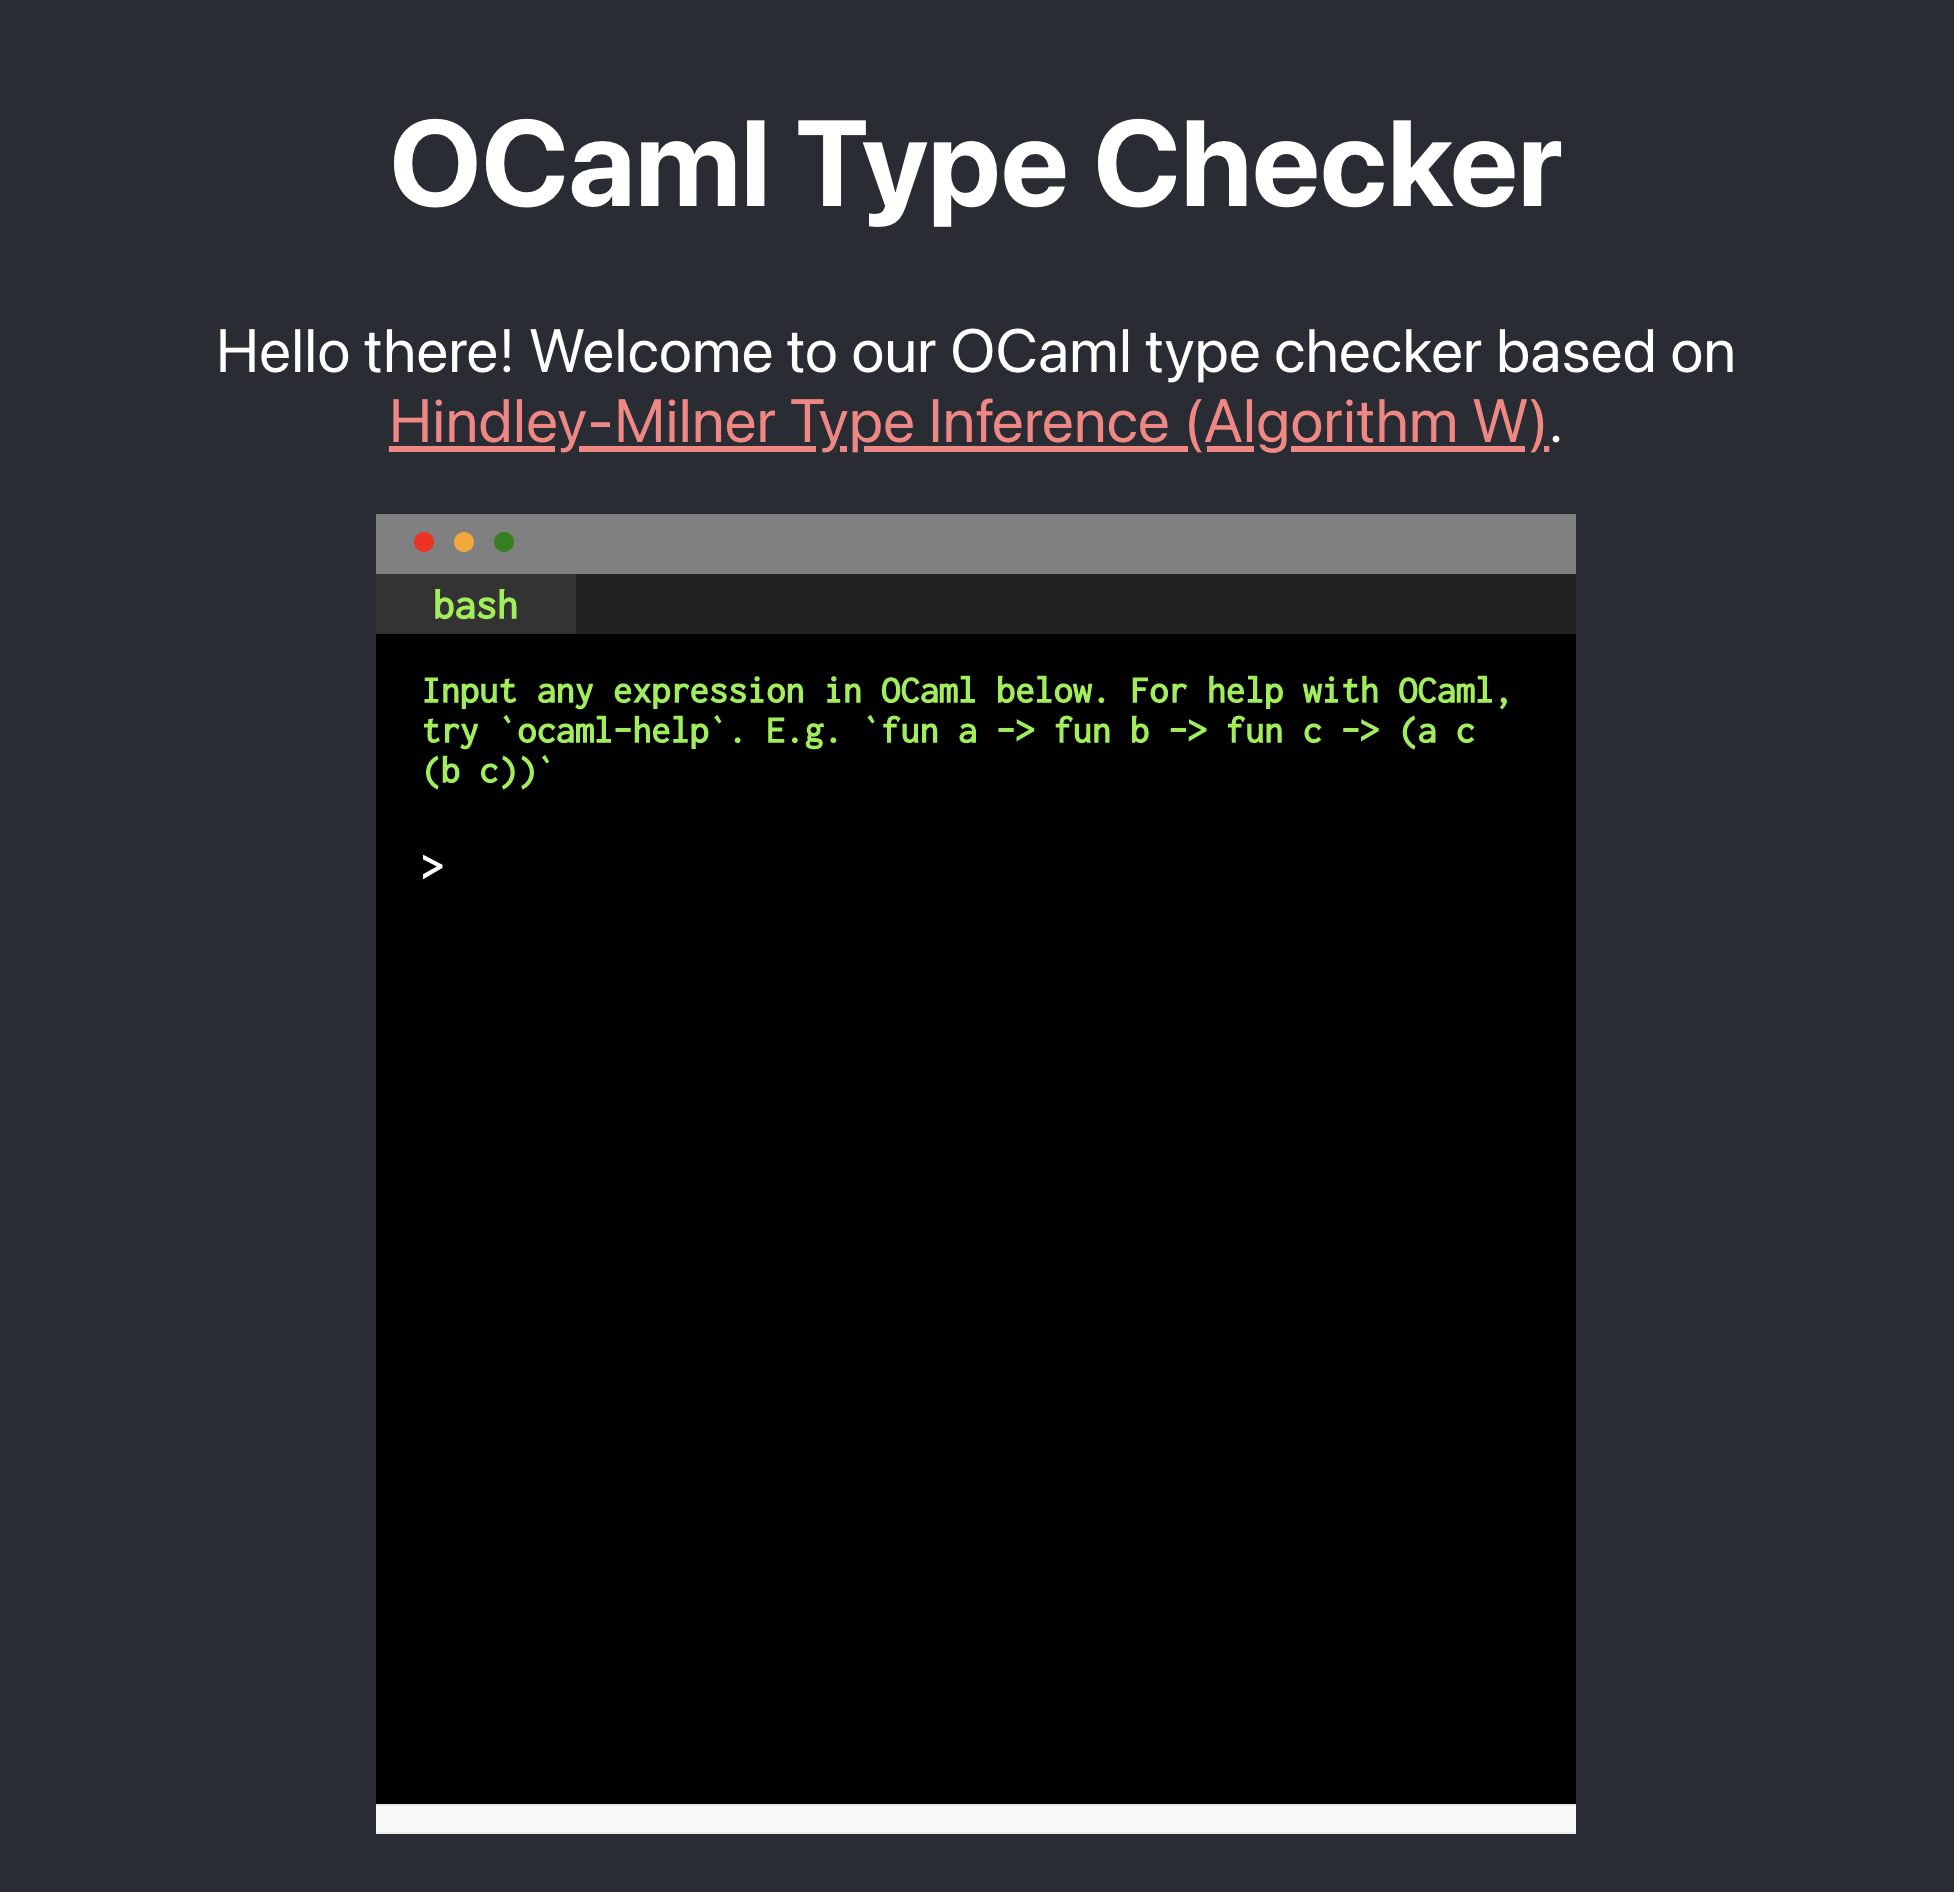
\includegraphics[width=0.8\linewidth]{images/frontend-ui.png}}
\caption{Frontend user interface}
\label{fig}
\end{figure}

\subsection{Architecture}
Figure \ref{fig:architecture} below provides an overview of the overall architecture of the project. The user input via the browser-based frontend is first accepted and put through our antlr4ts-enabled parsing process. This ends in the creation of a parse tree with custom AST Nodes, which we then feed into our Hindley-Milner type inference algorithm as detailed in earlier sections. The output is then either a valid type inference output that contains polymorphic type symbols (e.g. t0), or an error output (e.g. Inference Error).
\begin{figure}[H]
\centerline{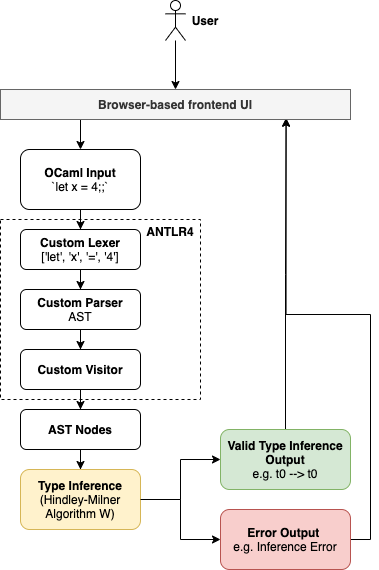
\includegraphics[width=0.6\linewidth]{images/architecture.png}}
\caption{Application architecture overview}
\label{fig:architecture}
\end{figure}
